
\documentclass[template=tabling,81pt,headonall]{azmoon}
\usepackage{xepersian}
\usepackage{amsfonts}
\usepackage{graphicx}
\usepackage{svg}
\svgpath{ {./images/} }
\graphicspath{ {./images/} }
\settextfont{Yas}
\setdigitfont{A Iranian Sans}
\usepackage{fontawesome5}

\printanswers
    \teacher{محمد صالح علی اکبری}
    \teachertitle{دبیر}
    \city{گناباد}
    \schooltitle{دبستان}
    \school{پیشگامان ظهور}
    \grade{چهارم}
    \branch{۱}
    \topic{ریاضی}
    \examdate{مهر ۱۴۰۶}
    \answertime{۹۰ دقیقه}
    \begin{document}
	\begin{questions}
		\nointerlineskip%
		\vskip-\baselineskip
		\question[1]{%
درست یا نادرست بودن هر یک از عبارت‌های زیر را مشخص کنید.
    \begin{parts}[1]\part{در عدد $507083002$ عدد $7$ در مرتبه یکان طبقه میلیون قرار دارد. \hfill (\qquad\qquad)}
\part{$423$ ثانیه برابر $8 \dfrac{12}{60}$ دقیقه است که به طور تقریبی آن را $8$ دقیقه در نظر می‌گیریم. \hfill (\qquad\qquad)}
\part{به متوازی الاضلاعی که زاویه‌های برابر داشته باشد، لوزی می‌گویند. \hfill (\qquad\qquad)}
\part{عدد $1680$ بر عدد های $7,5,3,2$ بخش پذیر است. \hfill (\qquad\qquad)}
\end{parts}

    }\question[1.75]{%
در جاهای خالی کلمه مناسب بنویسید.
    \begin{parts}[1]\part{۵ تا چک پول ۵۰۰ هزار ریالی برابر ...... ریال با ........ تومان}
\part{اگر دو کسر صورت های برابر داشته باشند کسری کوچک تر است که مخرج .......... باشد.}
\part{$3/5$ یعنی ......... تا $0/1$ و ......... $72$ تا $0/1$ می‌باشد.}
\part{در هر متوازی الاضلاع اندازه ......... روبه‌رو با هم مساوی و ...... روبه‌رو با هم موازی هستند.}
\end{parts}

    }\question[0.5]{%
گزینه صحیح را در هر مورد مشخص کنید: \\[0.3em]
\textbf{۱)} مثلث (م د ج) مثلث متساوی‌الاضلاع است. اندازه زاویه مشخص شده چند درجه است؟ \\
\parbox[c]{0.65\textwidth}{%
\begin{fourchoice}[1]
\choice{$25$ درجه}
\choice{$30$ درجه}
\choice{$35$ درجه}
\choice{$40$ درجه}
\end{fourchoice}%
}\hfill%
\\\\ \parbox[c]{0.3\textwidth}{\centering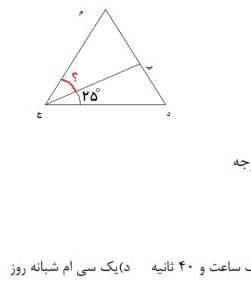
\includegraphics[scale=0.25]{chaharom_q3_mosalas}} \\[0.5em]
\textbf{۲)} کدام یک از زمان‌های زیر از بقیه طولانی‌تر است؟
\begin{fourchoice}[2]
\choice{$679$ ثانیه}
\choice{$12$ دقیقه و $30$ ثانیه}
\choice{خمس یک ساعت و $40$ ثانیه}
\choice{یک سی‌ام شبانه‌روز}
\end{fourchoice}}\question[1]{%
با توجه به عدد زیر به سوالات پاسخ دهید: \hfill \textbf{\large 89147256}
    \begin{parts}[1]\part{این عدد را به حروف بنویسید: \dotfill}
\part{کدام رقم در مرتبه یکان هزار قرار دارد؟ \dotfill}
\part{ارزش مکانی عدد ۵ را بنویسید: \dotfill}
\part{این عدد را در جدول ارزش مکانی نشان دهید: \dotfill}
\end{parts}
‌
\\
    }\question[1]{%
در الگوی زیر شکل هشتم از چند دایره تشکیل شده است؟ (نوشتن رابطه الزامی است) \\[0.3em]
\centering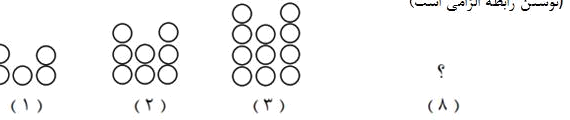
\includegraphics[scale=0.35]{chaharom_q5_olgoo} \\[0.3em]
\raggedright رابطه یا فرمول: \dotfill‌
\\}\question[1.5]{%
مقایسه کنید ($>$ یا $<$ یا $=$):
    \begin{parts}[3]\part{$3256 \quad \bigcirc \quad 479$}
\part{$\dfrac{3}{5} \quad \bigcirc \quad \dfrac{3}{8}$}
\part{$\dfrac{2}{3} \quad \bigcirc \quad \dfrac{5}{12}$}
‌\\\part{$3\dfrac{3}{4} \quad \bigcirc \quad 3\dfrac{2}{4}$}
\part{$6\dfrac{8}{12} \quad \bigcirc \quad 9\dfrac{3}{6}$}
\part{$7/1 \quad \bigcirc \quad 6/4$}
\end{parts}

    }\question[1]{%
کسرهای زیر را ساده کنید:
    \begin{parts}[2]\part{$\dfrac{12}{20} = $}
\part{$\dfrac{14}{21} = $}
\end{parts}
‌
\\
    }\question[1]{%
کیف فیروزه $4/2$ کیلوگرم و کیف دوستش $3/9$ کیلوگرم وزن دارد. وزن کیف فیروزه چند کیلوگرم بیشتر از وزن کیف دوستش می‌باشد؟‌
\\‌
\\}\question[1]{%
کشاورزی $\dfrac{3}{6}$ مزرعه‌ی خود را گل آفتابگردان و $\dfrac{3}{18}$ آن را گل رز کاشته است:
    \begin{parts}[1]\part{چه کسری از زمین را گل کاشته است؟}
‌\\\part{چه کسری از زمین بدون کشت مانده است؟}
\end{parts}
‌
\\
    }\question[2]{%
حاصل ضرب و تقسیم زیر را به دست آورید: \\[0.3em]
\centering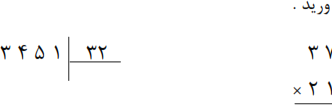
\includegraphics[scale=0.38]{chaharom_q10_zarb_taghsim}‌
\\‌
\\}\question[2]{%
برای هر شکل مقدار (؟) را به دست آورید: \\[0.3em]
\centering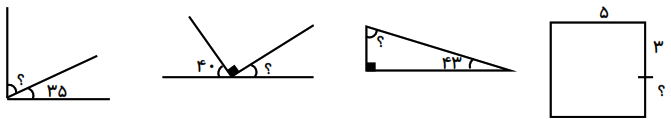
\includegraphics[scale=0.4]{chaharom_q11_zaviyeha}‌
\\}\question[2]{%
مساحت قسمت رنگی را به دست آورید: \\[0.3em]
\centering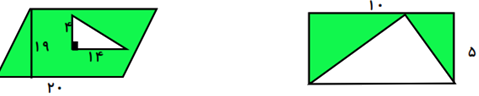
\includegraphics[scale=0.45]{chaharom_q12_shekl}‌
\\‌
\\}\question[2]{%
یک زمین کشاورزی مستطیل شکل به طول $20$ متر و عرض $15$ متر داریم. می‌خواهیم دور این زمین را نرده بکشیم به چند متر نرده نیاز داریم؟ اگر برای هر متر مربع از این زمین کشاورزی $3$ کیلوگرم بذر گندم نیاز باشد چند کیلوگرم بذر گندم برای همه‌ی زمین لازم است؟‌
\\‌
\\‌
\\}\question[0.75]{%
تاسی را پرتاب می‌کنیم. برای هر یک از احتمالات زیر یک جمله بنویسید:
    \begin{parts}[1]\part{احتمال آمدن عدد زوج؟ \dotfill}
\part{احتمال آمدن عدد دورقمی؟ \dotfill}
\part{احتمال آمدن عدد کمتر از ۷؟ \dotfill}
\end{parts}

    }\question[1]{%
قیمت نفت در ۵ هفته گذشته به صورت زیر بوده است: \\[0.3em]
\noindent
\begin{tabular}{|c|c|c|c|c|c|}
\hline
هفته & ۱ & ۲ & ۳ & ۴ & ۵ \\ \hline
قیمت & ۱۰۵ & ۱۰۷ & ۱۰۹ & ۱۱۰ & ۱۰۸ \\ \hline
\end{tabular} \\[0.5em]
الف) نمودار خط شکسته مربوط به آن را رسم کنید. \\
ب) در کدام هفته‌ها قیمت کمترین و بیشترین مقدار بوده است؟ \dotfill \\
ج) تغییرات قیمت نفت در کدام هفته از بقیه هفته‌ها کمتر است؟ \dotfill‌
\\‌
\\‌
\\}\question[0.5]{%
عددهای داده شده را با تقریب‌های خواسته شده بنویسید:
    \begin{parts}[2]\part{$476$ با تقریب در دهگان $\longrightarrow$ \dotfill}
\part{$23162$ با تقریب در هزارگان $\longrightarrow$ \dotfill}
\end{parts}

    }\end{questions}
    \end{document}
    